\section{Testing Estructural (Caja Blanca)}

Sirve para testear programas secuenciales, con un \'unico punto de ingreso y un \'unico punto de terminaci\'on.

Una ejecuci\'on del programa que termina satisfactoriamente, est\'a asociada a un \textbf{camino completo} en el flowgraph del programa (va desde el nodo inicial hasta el nodo asociado a la terminaci\'on). 

Un \textbf{camino no factible} es aquel que no puede ser realizado porque es l\'ogicamente imposible. 

Proceso para hacer un test estructural: 

\begin{enumerate}
 \item Con el c\'odigo como base, dibujamos el grafo de flujo de control 
 \item Determinamos el conjunto de todos los caminos completos.
 \item Preparamos los datos de test que forzar\'an la ejecuci\'on de cada camino. Para ello hay que conseguir conjunto de valores de entrada tal que: 
  \begin{enumerate}[(a)]
    \item Cubra todas las sentencias (nodos del flowgraph).
    \item Cubra todos los branches (ejes del flowgraph). 
    \item Cubra todos los casos (True y False) de las condiciones.  
    \item Cubra todas las duas (terna $[d,u,x]$ tal que: $d$ es un nodo que tiene la definici\'on de la variable $x$, $u$ es un nodo o arco en donde se usa $x$, y hay al menos un camino desde $d$ hasta $u$ que no contiene otra definici\'on de $x$. 
    \item Cubra todos los dem\'as caminos que los incisos anteriores no cubren.
  \end{enumerate}
 \item Evaluamos que cada test cumpla con los criterios. 
 \item Eventualmente, iteramos hasta terminar con todos los tests hasta tener cubiertos todos los caminos. 
\end{enumerate}

Lo que buscamos testear ac\'a son todos los caminos que puede tomar un programa. Para ello hay que graficar el CFG, un grafo de flujo o \emph{flowgraph} que representa el flujo de control de un programa. 

\lstset{language=C++,numbers=left,showstringspaces=false}

\begin{table}[H]
\caption{Ejemplo de c\'odigo y CFG asociado}
%\lstset{linewidth=4.5cm}
\begin{tabular}{l l} 
\begin{lstlisting}
void calculo(int x, int y) {
  int w = 0;
  if( x%2 == 0 ){
    w = 21;
  }else{
    w = 31;
  }
  int z = x + y;
  if( z==0 || z==1 ){
    while( z<w ){
      z = z+10;
    }
  }
  if( z!=30 ){
    print( "no llegamos a 30" );
  }
}
\end{lstlisting} & 
\raisebox{-6cm}{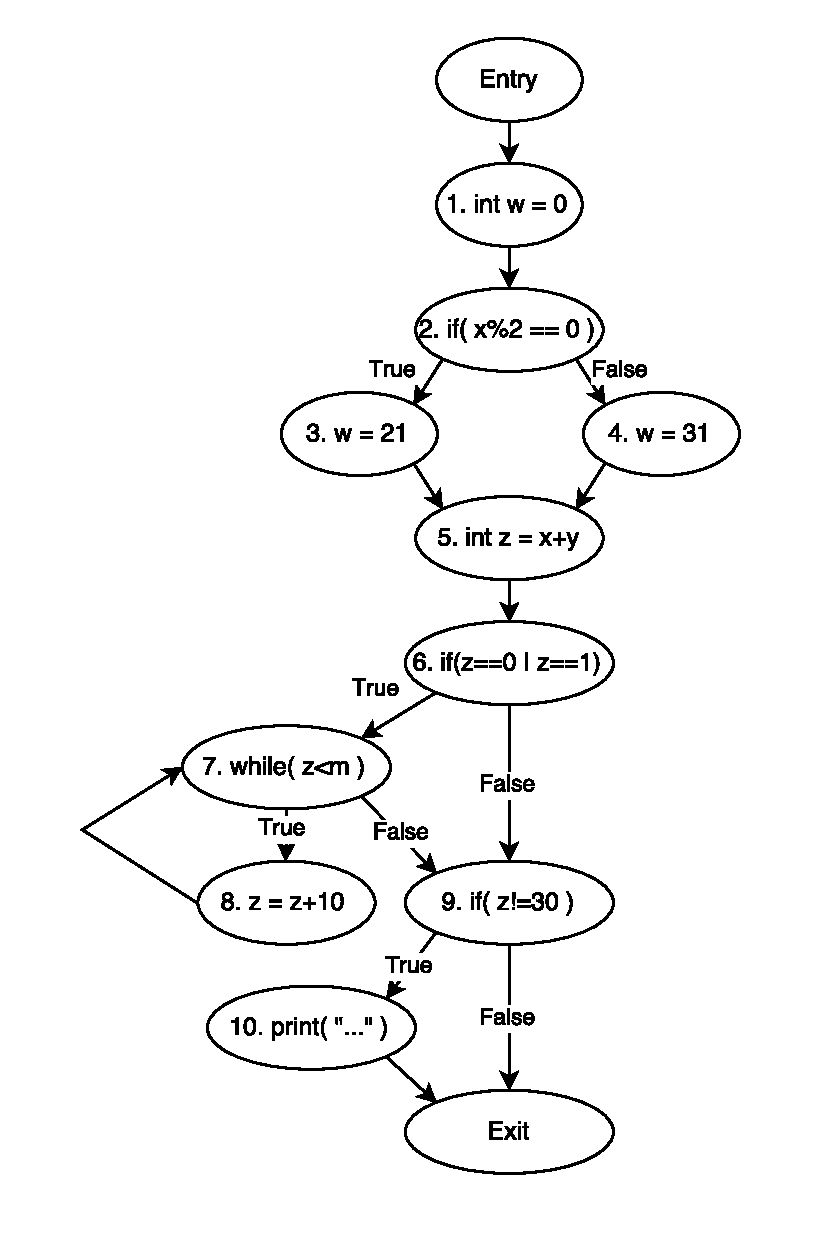
\includegraphics[width=7cm]{images/flowgraph_test_estructural.pdf}}
\end{tabular}
\end{table}


